%Outline
%\begin{itemize}
%	\item Graph definition
%	\item Agent definition
%	\item Solution
%	\begin{itemize}
%		\item Explanation: a pathlike object
%		\item Definition: (c$_1$ ... c$_n$)
%		\item Constraints: where c1 = start, cn = goal, legal transitions
%	\end{itemize}
%	\item Remaining formalization
%\end{itemize}



\section{Flatland}\label{sec:flatland}

\subsection{Environment}\label{sec:environment}
The environment is represented by a directed graph $G = (V,E)$, where $V$ is a finite set of vertices and $E$ is the set of edges that connect pairs of vertices.  For each edge $e \in E$, we define a triple $(C,D,\Delta)$, where:
\begin{itemize}
	\item $C$ is the directed pair of vertices that the edge connects
	\item $D$ is the set of valid traversal directions
	\item $\Delta$ is the resulting change in direction
\end{itemize}

\noindent Although the environment is represented here as a graph, its original form is a lattice grid comprising cells and tracks.  Cells represent locations where a train can be at any time step, and tracks dictate the connectedness of the cells---consequently, which cells a train can transition to.  Empty cells, which contain no track, are omitted from the graph.

\subsection{Trains}\label{sec:trains}
A train is an agent that traverses the graph.  Each train $t$ belongs to the set of trains $T$ and can be represented by the tuple $(S, G)$, where $S$ is the set of starting conditions and $G$ is the set of goal conditions.
\begin{itemize}
	\item each starting condition $s \in S$ is represented by a triple $(p,o,e)$, where $p$ is the starting position as a coordinate pair, $o$ is the starting direction, and $e$ is the earliest departure time
	\item each goal condition $g \in G$ is represented by a tuple $(p',a)$, where $p'$ is the target position as a coordinate pair and $a$ is the latest arrival time
\end{itemize}

\subsection{Solution}\label{sec:solution}
A valid solution candidate for a single train is a sequence of vertices $v_i \in V$ for $0 \leq i \leq n$ such that $(v_i,v_{i+1}) \in C$ for all $0 \leq i \leq n$.  Furthermore, it must be the case for a valid solution vandidate for a single train $t_a$ that:
\begin{itemize}
	\item $v_{1_a} = p_a$
	\item $v_{n_a} = p'_a$
\end{itemize}
\noindent In other words, the first vertex in the sequence corresponds to the starting position of the train and the final vertex in the sequence corresponds to the target position of the train.

\subsection{Example}\label{sec:example}
Vertices in the graph correspond to cells in the original Flatland grid.  The edges that connect pairs of vertices correspond to the tracks in the original Flatland grid.  

\begin{figure}
\centering
        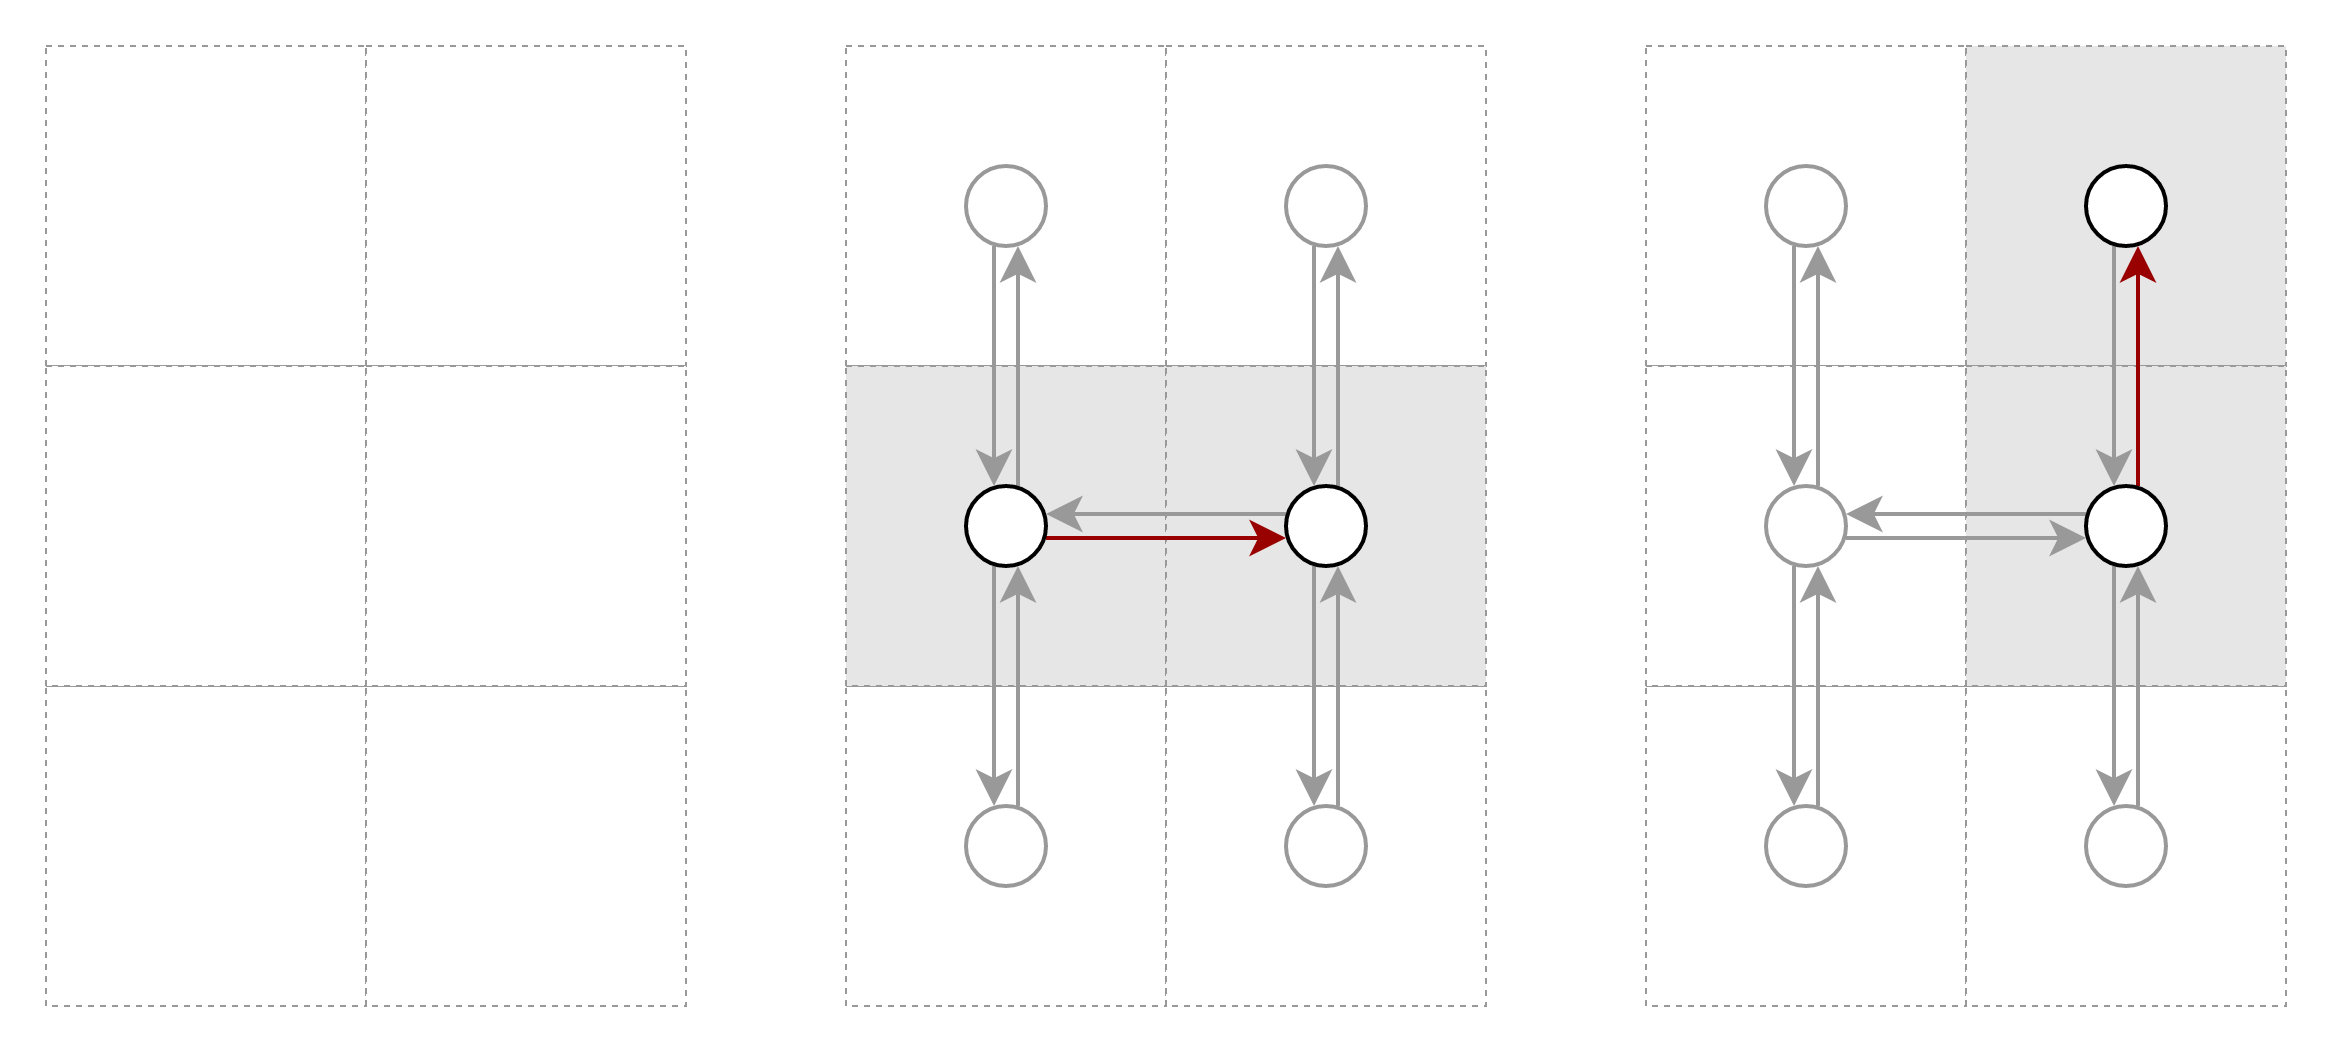
\includegraphics[width=\linewidth]{img/edges.png}
    \caption{Example}
    \label{fig:verticalcell}
\end{figure}

\begin{itemize}
	\item $(n_3 \rightarrow n_4, \{north\}, east)$
	\item $(n_4 \rightarrow n_2, \{north, east\}, north)$
\end{itemize}

\pagebreak

\section{Flatland}\label{sec:flatland}
The Flatland environment contains tracks and trains, which allows it to simulate the activity of a true railway network.  While the Flatland challenge represents the environment as a grid of height $h$ and width $w$, this paper will represent the environment as a graph.

\subsection{Environment}\label{sec:environment}
Consider $D = \{north,south,east,west\}$ the set of valid traversal directions and  $C = h \times w$ a set of \textit{cells}.
The environment is represented by a directed graph $G = (V,E)$, where $V = C \times D$ is a finite set of \textit{vertices} and $E \subseteq V \times V$ is a set of \textit{edges}.
Each vertex $v \in V$ corresponds to a cell $c \in C$ in the original Flatland grid and traversal direction $d \in D$, such that it can uniquely represented by the tuple $(c,d)$.
The Flatland simulation represents time as a finite series of discrete steps.

% A vertex $v \in V$

% Each cell corresponds to four vertices, each of which in turn corresponds to one of the four traversal directions in $D$.

\subsection{Trains}\label{sec:trains}
Each environment has $n$ number of trains, denoted by the set $Z = \{z_0,...,z_{n-1}\}$.  A train $z = (v_{start}, t_{depart}, F, t_{arrive})$ where:
\begin{itemize}
	\item $v_{start} \in V$ is the starting vertex
	\item $t_{depart}$ is the earliest departure time
	\item $F \subseteq V$ is the set of valid target vertices corresponding to the target position
	\item $t_{arrive}$ is the latest arrival time
\end{itemize}

\noindent is an agent that traverses the graph.

\subsection{Solution}\label{sec:solution}
A valid solution candidate for a single train $z \in Z$ is a sequence of vertices $v_i \in V$ for $0 \leq i < n$ such that $(v_i,v_{i+1}) \in E$ for all $0 \leq i \leq n$, as well as that $v_{0} = v_{start}$ and $v_{n} \in F$.  
The first vertex in the sequence corresponds to the starting vertex of the train, whereas the final vertex in the sequence corresponds to one of the valid target positions of the train.


\subsection{Example}\label{sec:example}
Vertices in the graph correspond to cells in the original Flatland grid.  
The edges that connect pairs of vertices correspond to the tracks in the original Flatland grid.  

\pagebreak

\section{Problem definition}\label{sec:problem_definition}
Consider the set of traversal directions $D = \{north, south, east, west\}$  and a list of $m$ cells $C = (c_1, ..., c_m)$. 
The Flatland environment is defined as a tuple $(G,A)$ in which $G$ is a directed graph $G = (V,E)$, such that $V = C \times D$ and $E \subseteq V \times V$, and $A$ is a list of $n$ agents $A = (a_1, ..., a_n)$.
Each agent $a_i \in A$ is associated with a start vertex $s_i \in V$ and a set of target vertices $T \subset V$.
Time is considered discrete; between two consecutive timesteps, an agent can either move to another vertex (move action) or stay at its current vertex (wait action).  
Additionally, each agent $a_i$ is assigned a departure time $\delta_i$ and an arrival time $\alpha_i$; it is between only these time steps that the agent is permitted to execute move actions.
A valid solution path $\pi_i$ of agent $a_i$ is a finite sequence $(v_j)_{j=1}^k$ of vertices $v_j \in V$ for $0 \leq j \leq k$ such that $(v_j,v_{j+1}) \in E$ for all $0 \leq j \leq k$, as well as that $v_1 = s_i$ and $v_k \in T$.
